\ProjectEntry
{Mixing Configurations for Downstream Prediction}
{First Author, Research Assistant with Prof. Shixin Xu}
{Python, PyTorch, Unsupervised Learning}
{
  \bitem{Proposed GraMixC: a configuration\,–\,mixing module that fuses unsupervised ``configurations'' with task predictors for label\,–\,efficient downstream performance.}
  \bitem{Defined configuration extraction and mixing objectives, and integrated them with linear probing / 3LP predictors without changing the backbone.}
  \bitem{Validated on DSNI regression (pH/temperature) and image benchmarks; figures show attention maps, lineage diagrams, and quantitative gains.}
  \bitem{Ablation demonstrates incremental mixing (GMC) outperforms static concatenation (GC).}
  \bitem{Co-authored with Hao Wu, Runkun Guo, Yihan Wang, Dongmian Zou, and Prof. Shixin Xu; under ICLR 2026 review.}
}
{assets/1004_gramixc/framework.png}
{\extlink{https://arxiv.org/abs/2510.19248}{arXiv preprint}}
{\badge{Unsupervised Learning} \badge{ICLR under review}}


\textbf{Technical Highlights:}
This project tackles the challenge of learning meaningful representations from unlabeled data by mixing configurations in a learned latent space. The key innovation is a training objective that encourages the model to predict properties of mixed configurations based on the mixing coefficients and component configurations.

\begin{figure}[ht]
  \centering
  \subcaptionbox{Configurations\label{fig:cifar10_linage}}{
    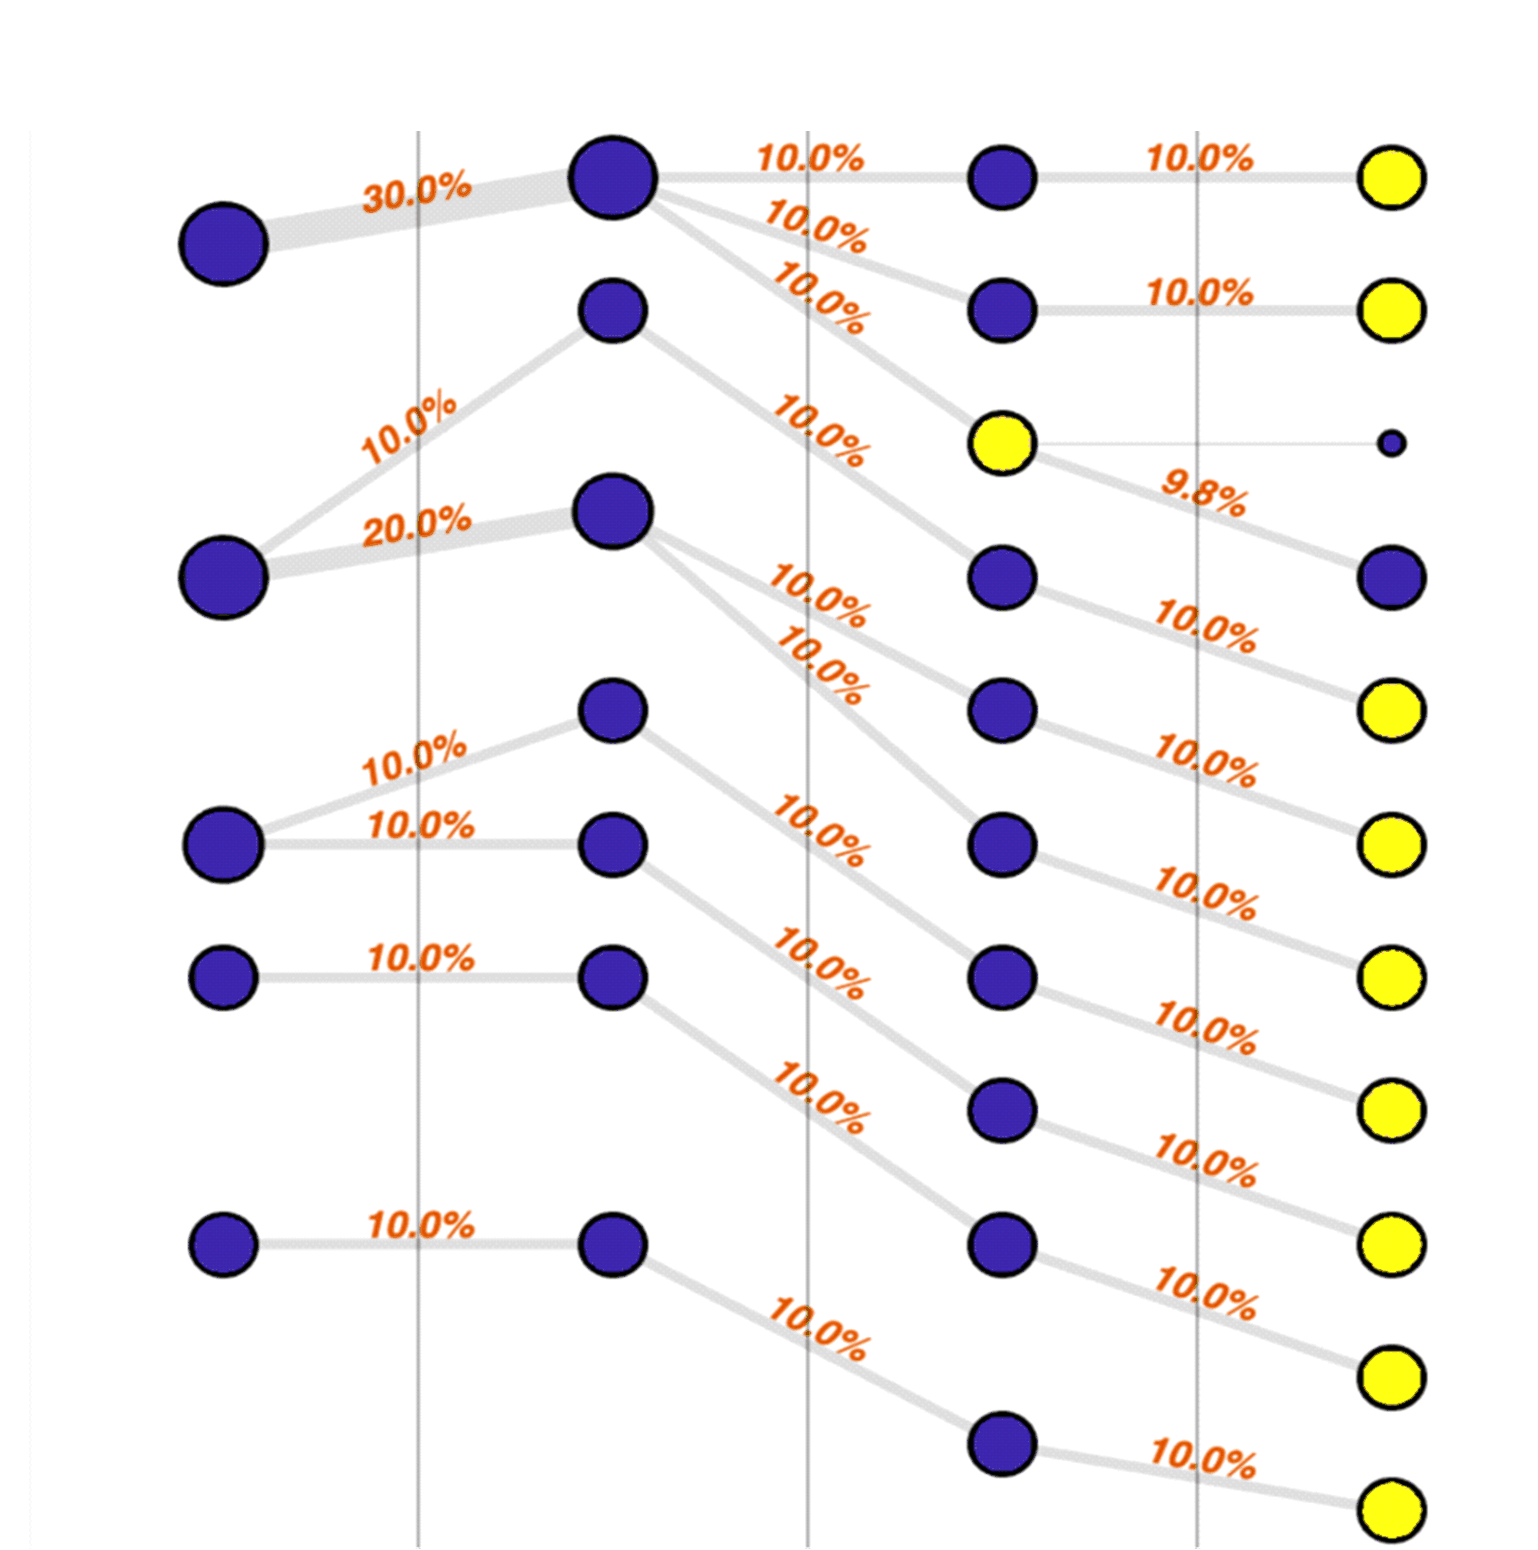
\includegraphics[width=0.2\linewidth]{assets/1004_gramixc/2.1.png}
  }
  \subcaptionbox{Cfg. attention map\label{fig:cifar10_GraMixC_attention}}{
    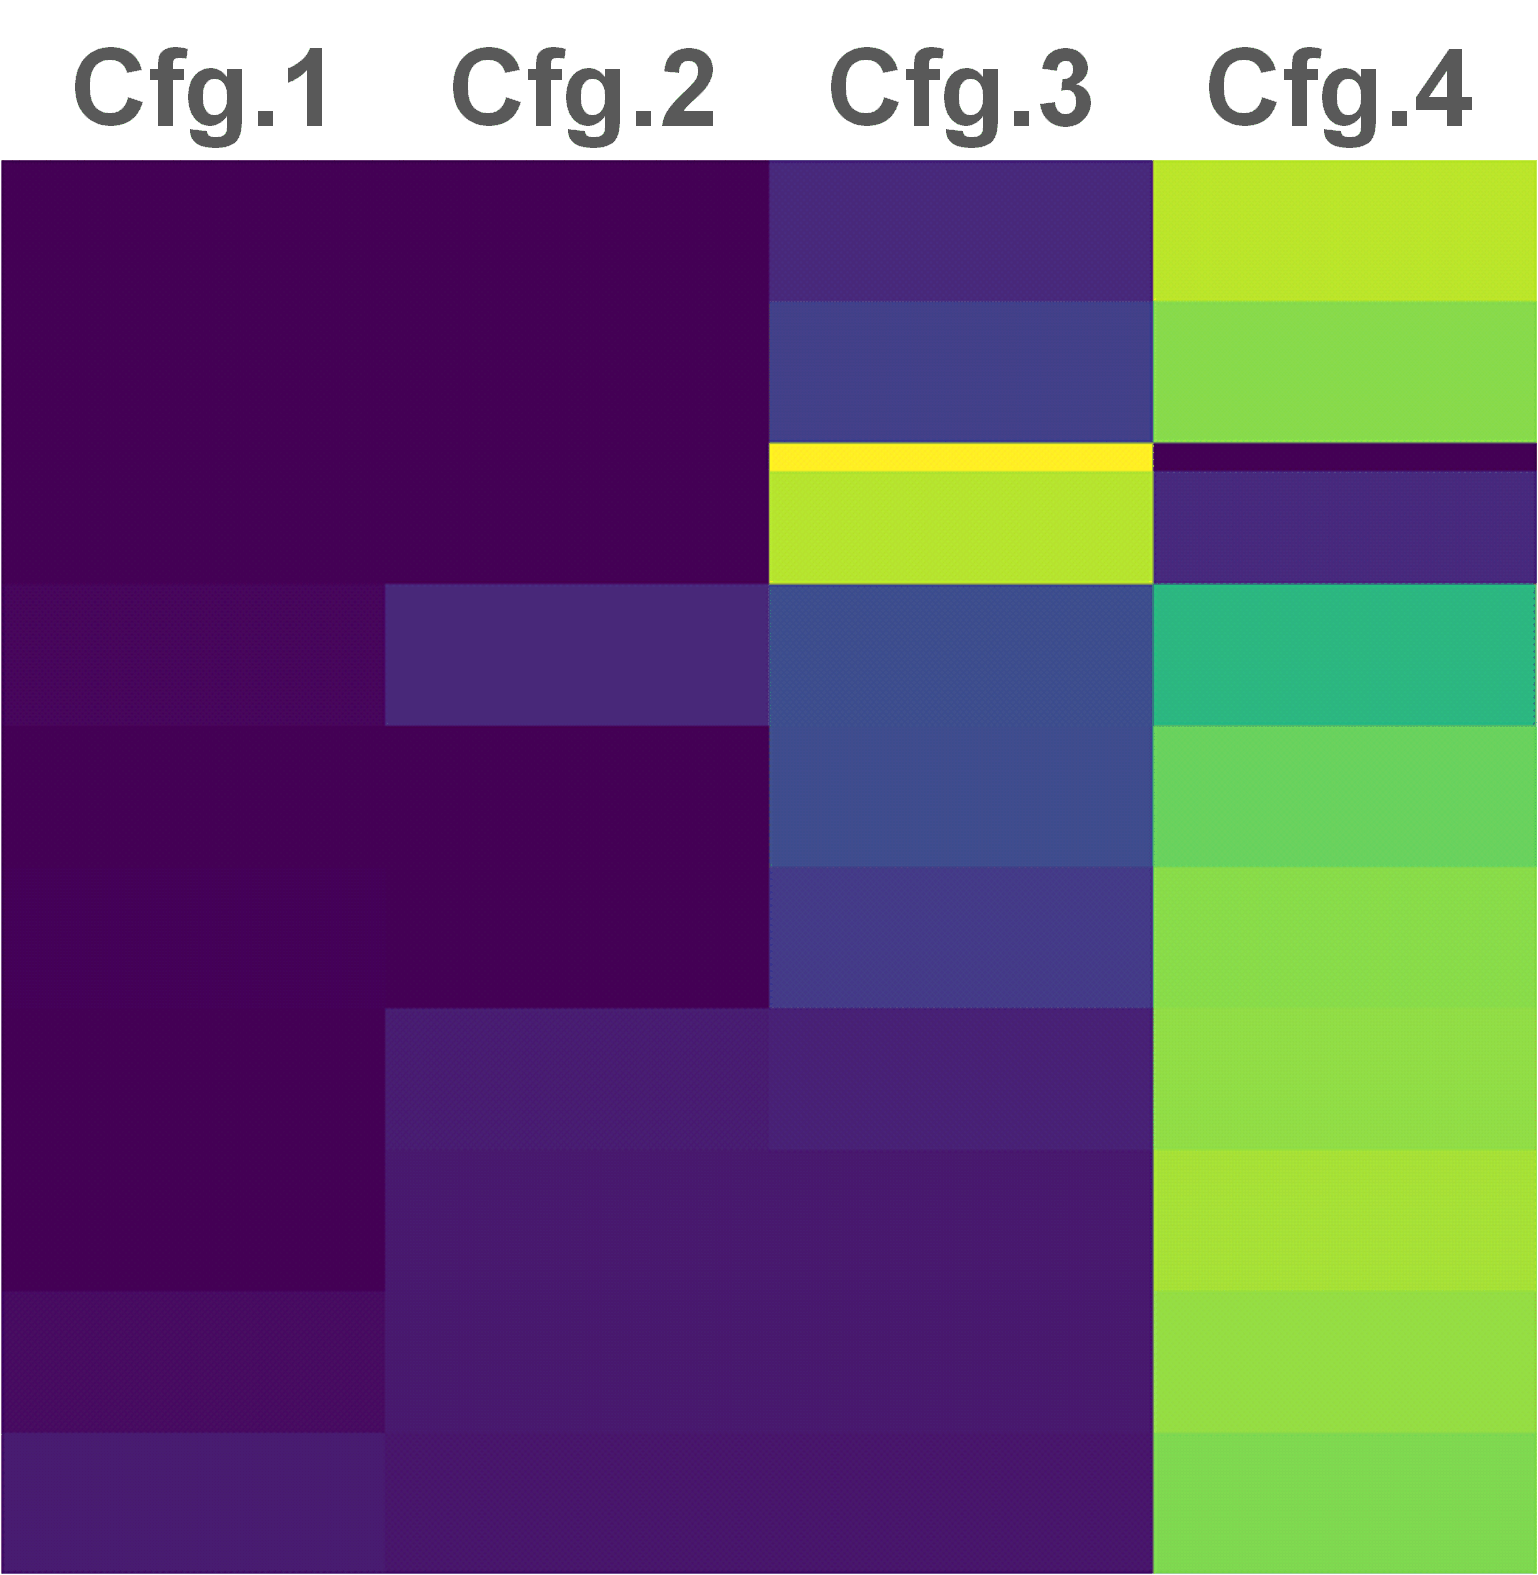
\includegraphics[width=0.2\linewidth]{assets/1004_gramixc/2.2.png}
  }
  \subcaptionbox{Reg. attention map\label{fig:cifar10_dino+reg_attentionl}}{
    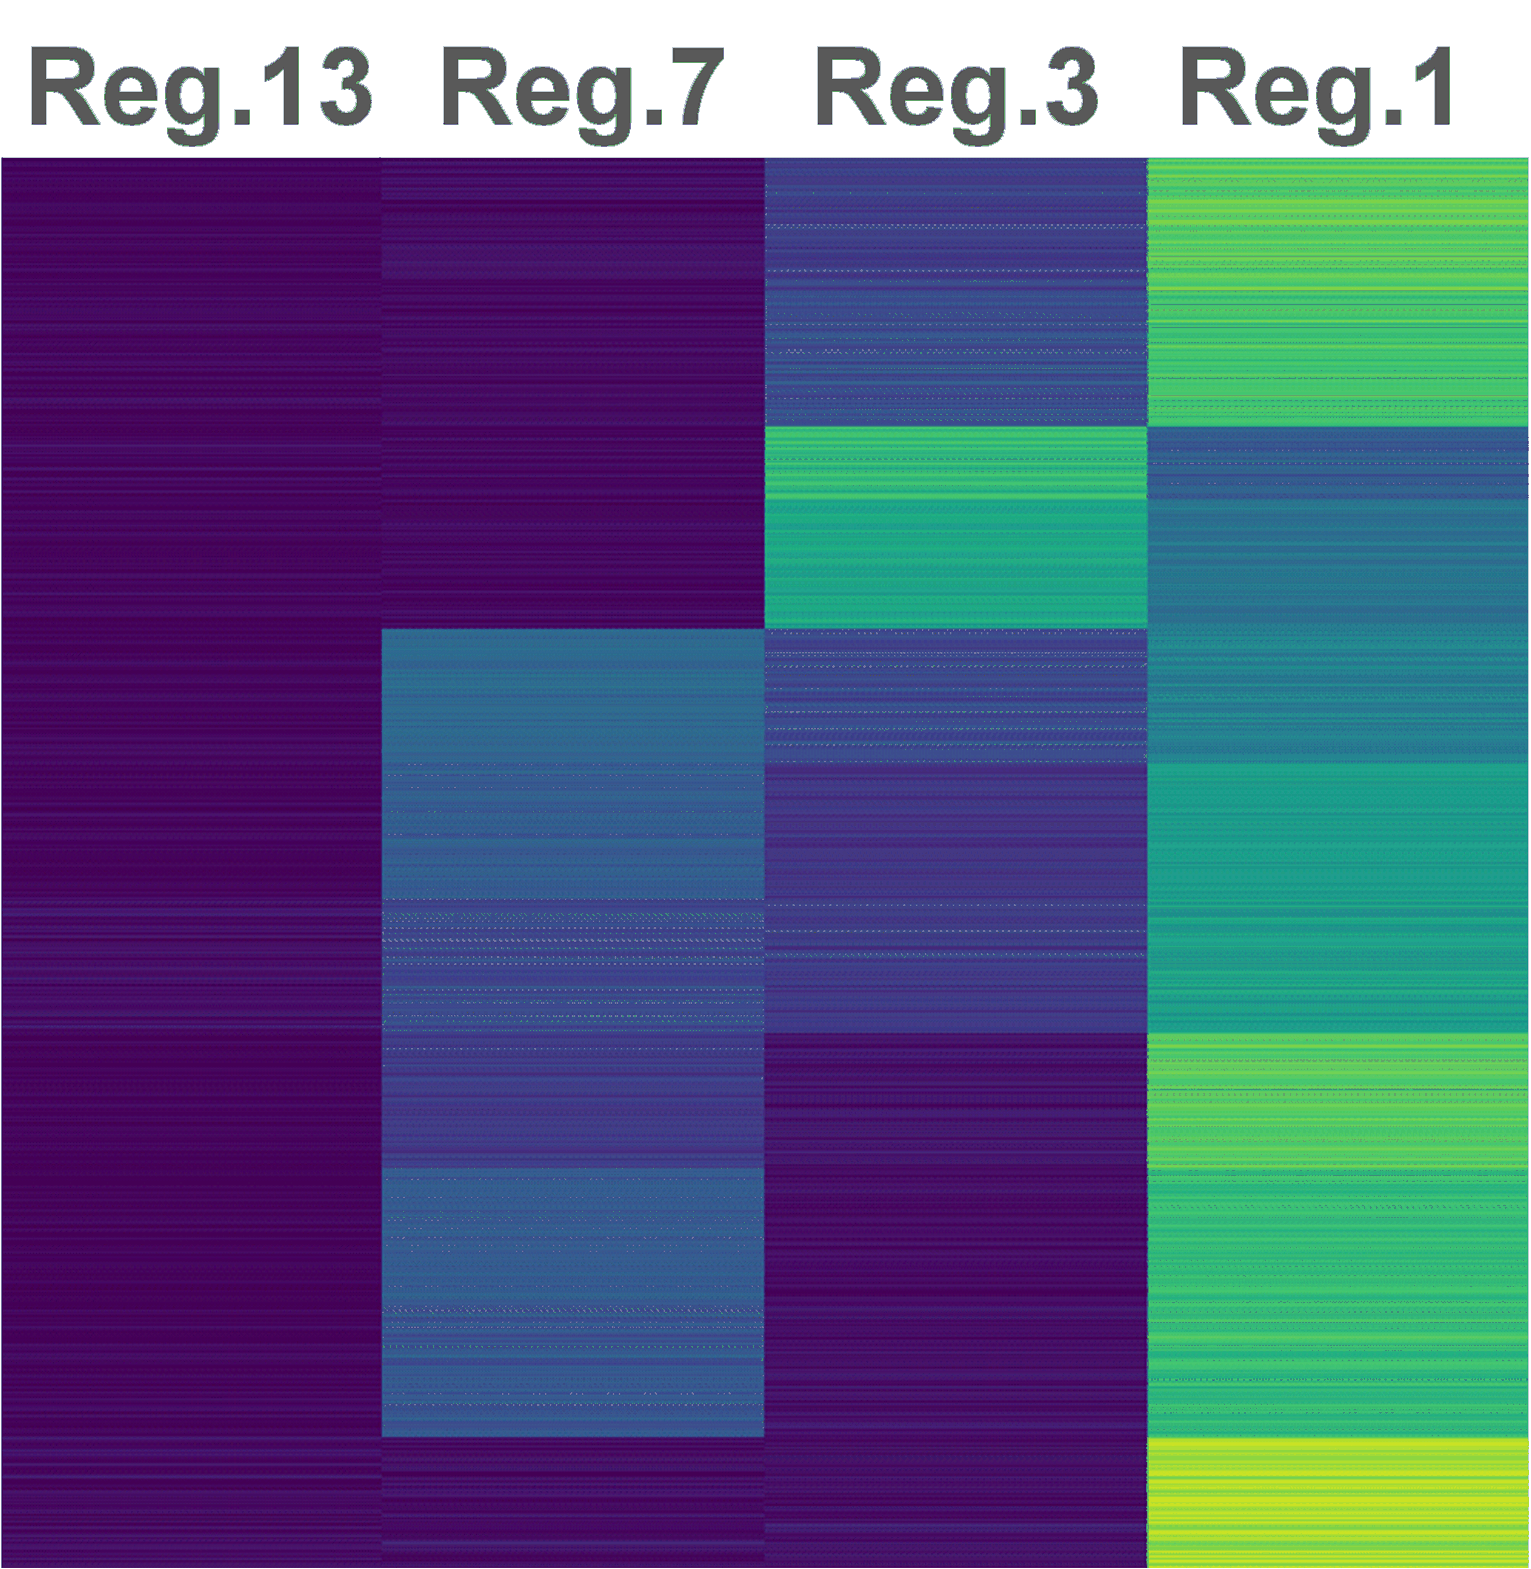
\includegraphics[width=0.2\linewidth]{assets/1004_gramixc/2.3.png}
  }
  \subcaptionbox{Reg. attention imgs\label{fig:cifar10_dino+reg_attentionl_map}}{
    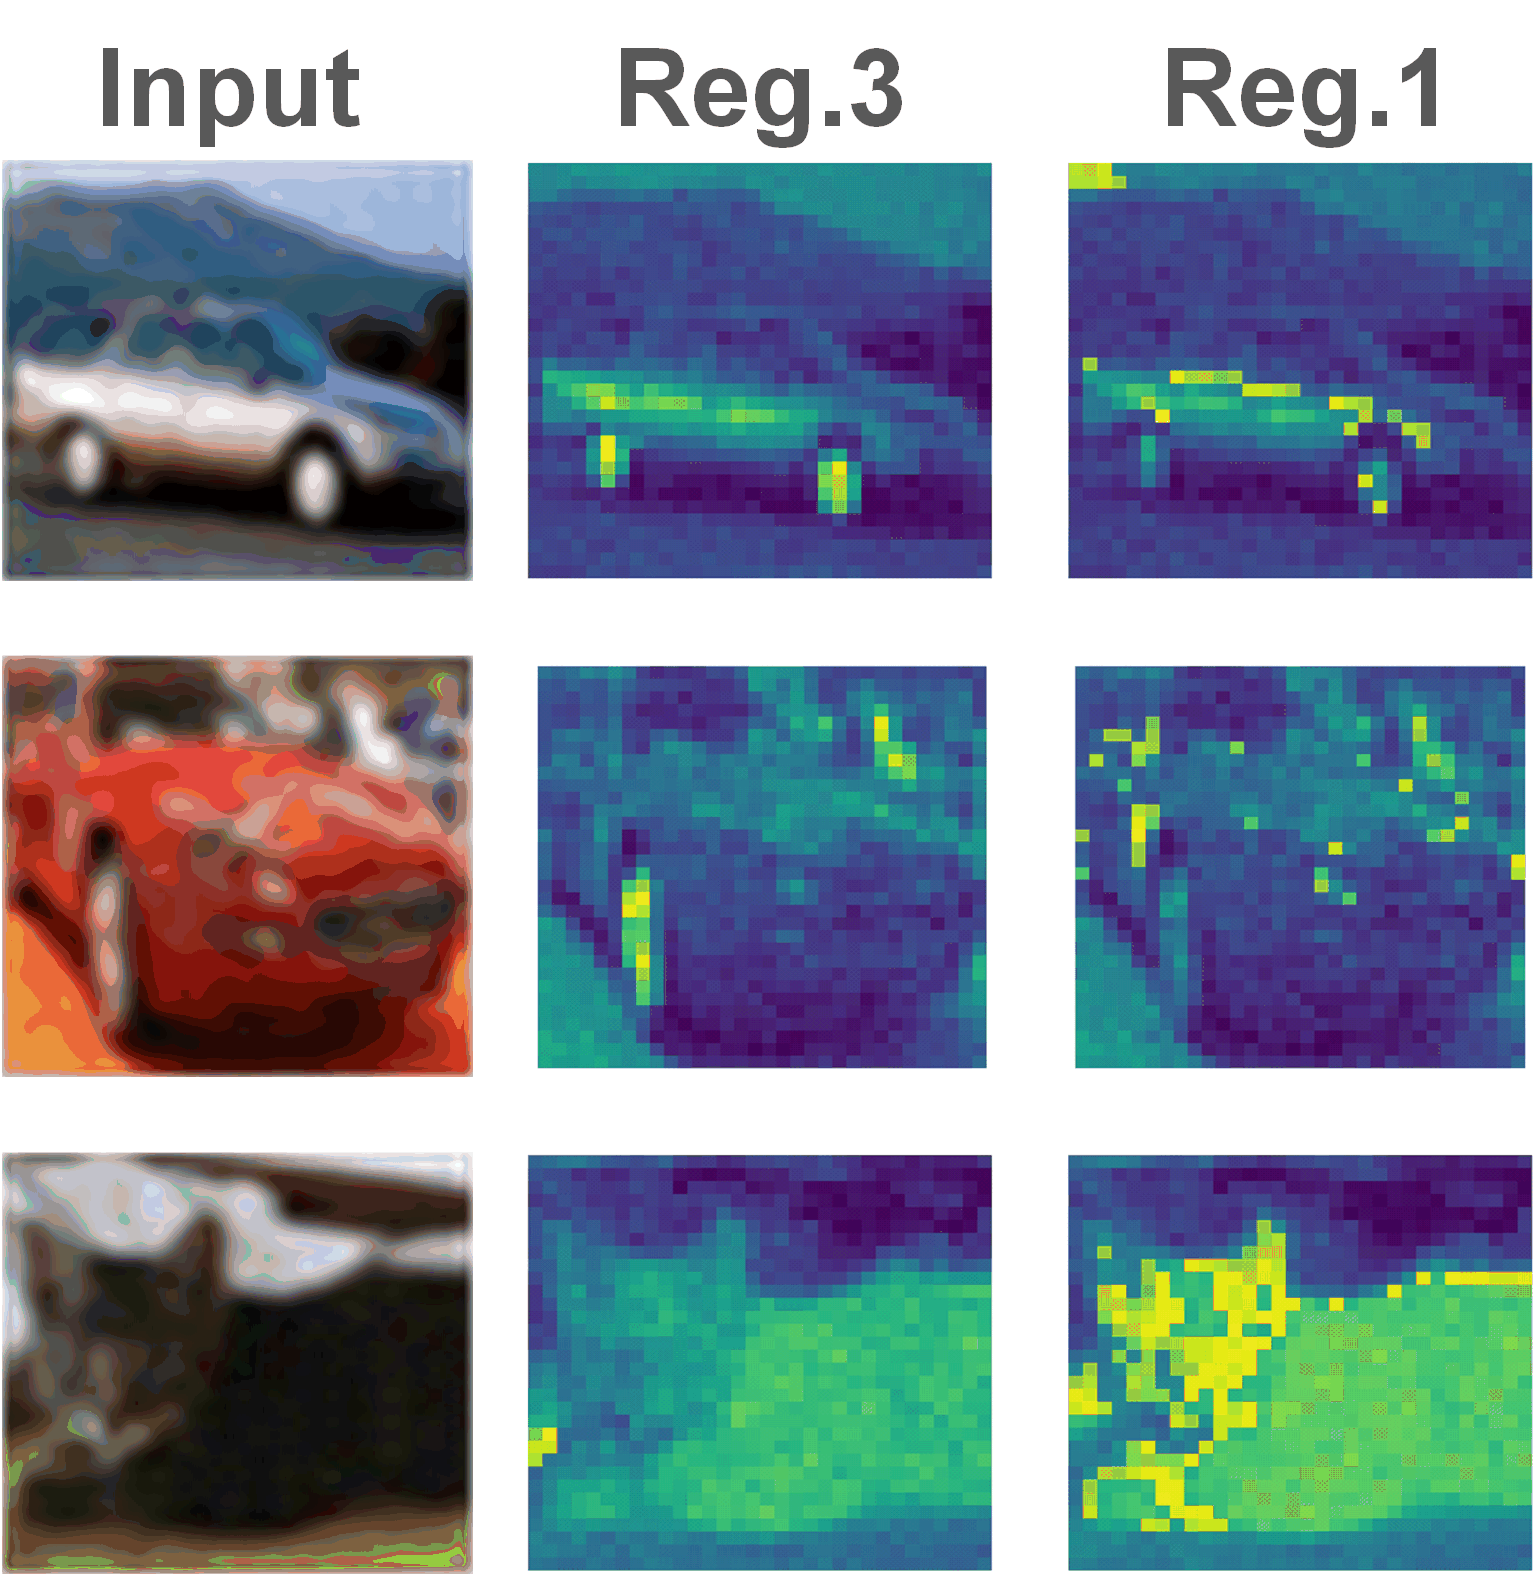
\includegraphics[width=0.2\linewidth]{assets/1004_gramixc/2.4.png}
  }
  \caption{
    Comparison of attention maps obtained from configurations and registers, rows for samples.
    \textbf{(a)}: Lineage diagram for configurations, near GT balls are marked yellow.
    \textbf{(b)}: Attention map of configuration tokens in an attention-based linear probing.
    \textbf{(c)}: Attention map of DINOv2-reg register tokens, mean of all patch norms is used.
    \textbf{(d)}: Attention maps over the register tokens, as images.
  }
  \label{fig:similar_behavior}
\end{figure}

\textbf{Key Results:}
\begin{itemize}[leftmargin=1.2em, itemsep=0.1em]
  \item Regression (DSNI): 3LP+GC improves over the 3LP baseline; 3LP+GMC further raises R$^2$ (up to $>0.9$), see Fig.~\ref{fig:dsmz_regression}.
  \item Ablation: Incrementally mixing configurations (GMC) consistently outperforms static train/test pairing (GC), Fig.~\ref{fig:dsmz_ablation}.
  \item Interpretability: Attention maps and lineage diagrams indicate configurations capture semantically meaningful structure (Fig.~\ref{fig:similar_behavior}).
  \item Design: GraMixC fuses configuration features with task predictors without modifying the backbone.
\end{itemize}


\textbf{Impact:} 
This work contributes to the growing field of self-supervised and unsupervised representation learning, with potential applications in materials science, molecular design, and any domain with configurable systems. Part of signature work research at Duke Kunshan University under Prof. Shixin Xu, focusing on unsupervised/semi-supervised methods for biomedical tasks.

\begin{figure}[ht]
  \centering
  \subcaptionbox{DSNI regression (3LP baseline vs. GC/GMC)\label{fig:dsmz_regression}}{
    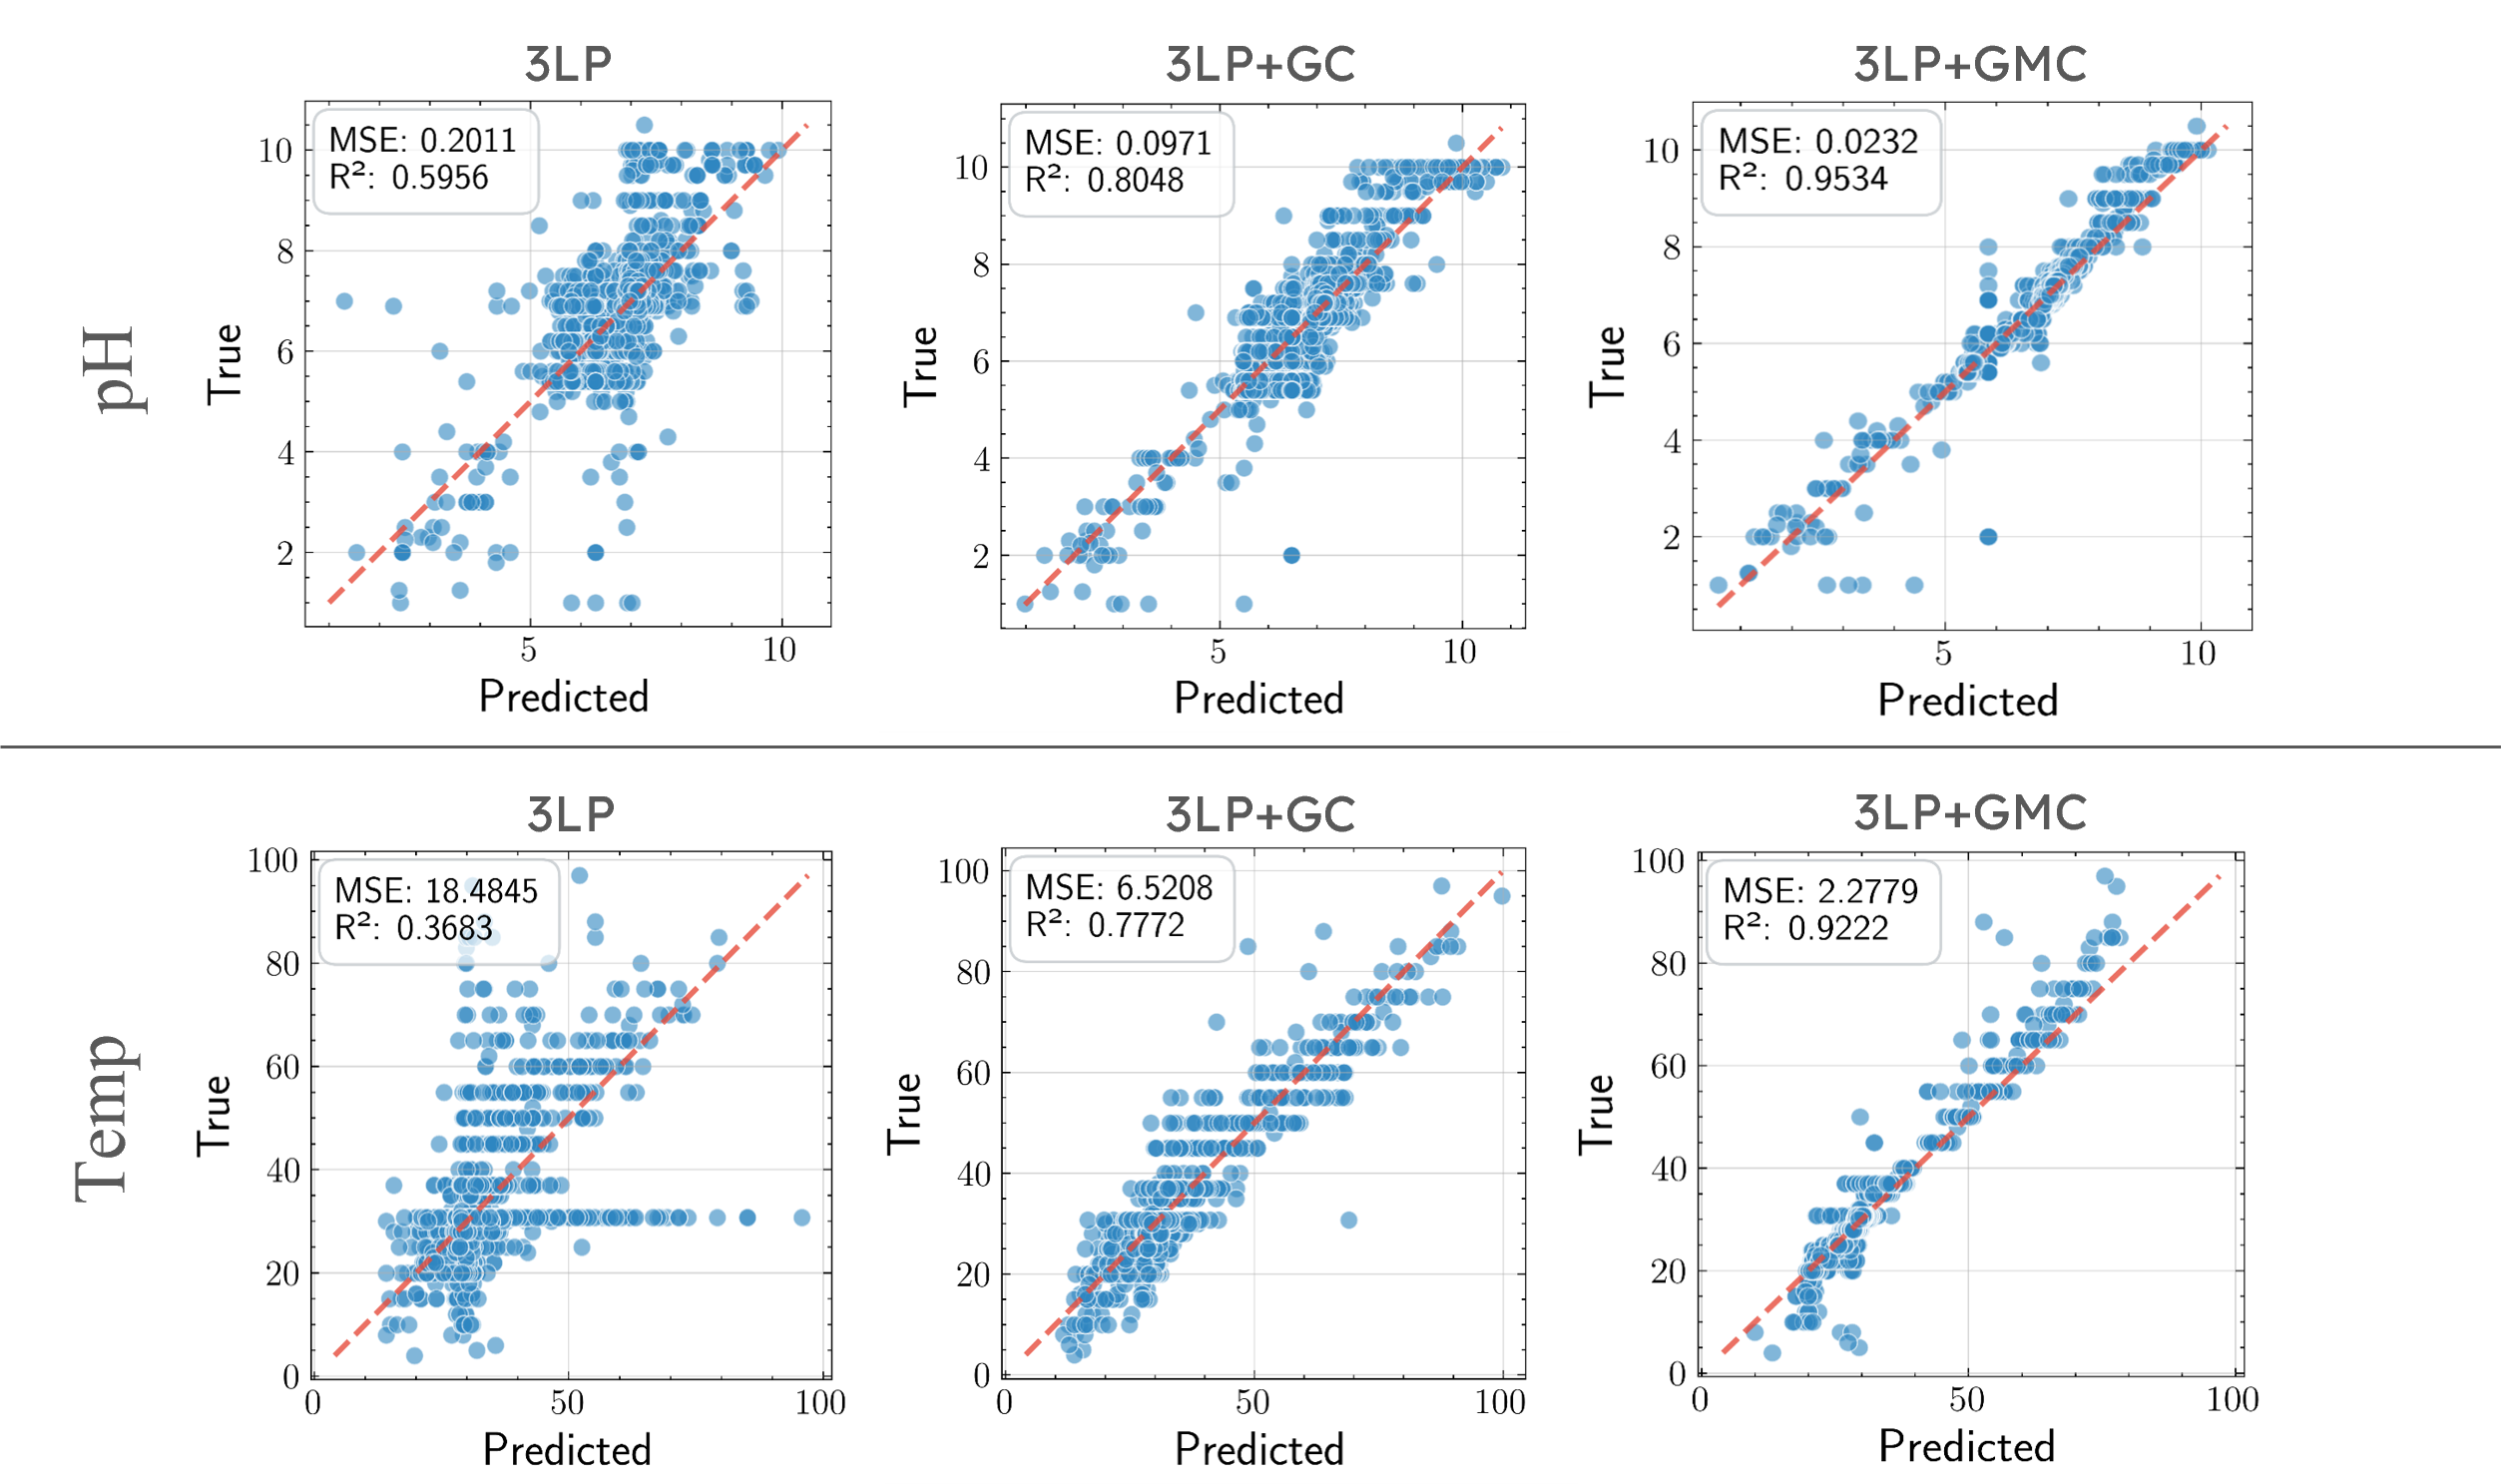
\includegraphics[width=0.48\linewidth]{assets/1004_gramixc/dsni_regression.png}
  }\hfill
  \subcaptionbox{DSNI ablation (mixing configurations)\label{fig:dsmz_ablation}}{
    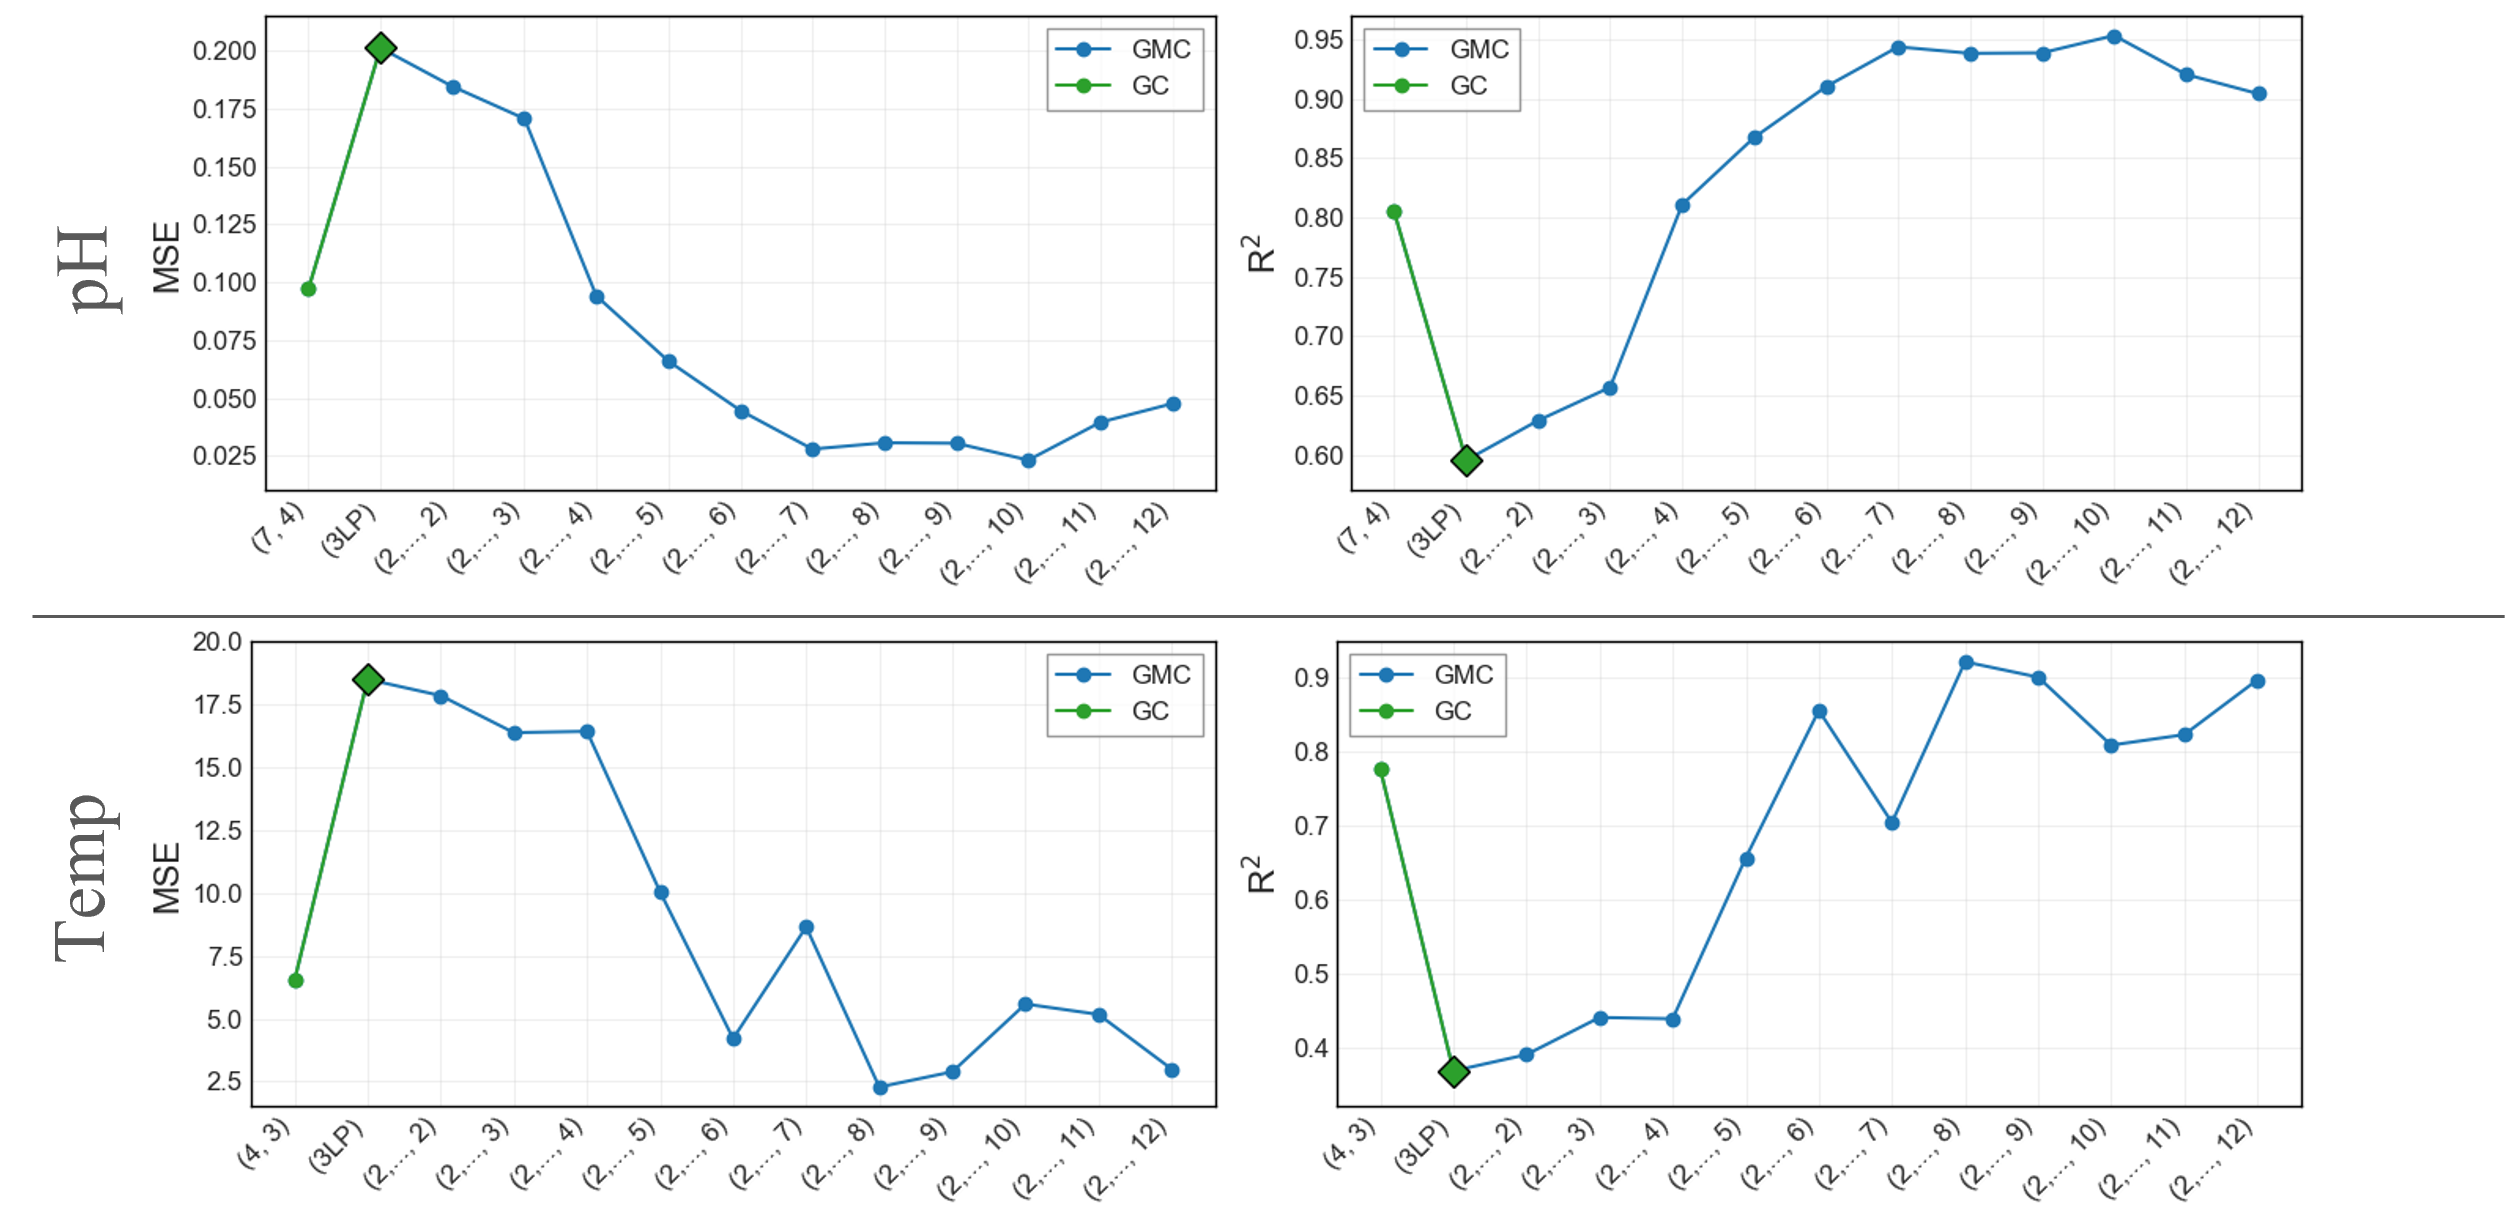
\includegraphics[width=0.48\linewidth]{assets/1004_gramixc/dsni_ablation.png}
  }
  \caption{Quantitative results on DSNI. (Left) Predicted vs. actual pH/temperature: 3LP+GC improves over 3LP; 3LP+GMC further increases R$^2$ (up to $>0.9$). (Right) Ablation: Incremental mixing (GMC) outperforms static train/test pairing (GC).}
\end{figure}